\documentclass[a4paper,12pt]{article}

\title{Physics 30 \\ Electric Forces \& Fields}
\author{Jad Chehimi}

% document setup
\renewcommand{\familydefault}{\sfdefault}
\linespread{1.25}
\usepackage[margin=1in]{geometry}
\usepackage{setspace}
\usepackage{enumitem}
\setlist{nosep}
\usepackage{color,soul}
\setcounter{secnumdepth}{0}

% tools
\usepackage[hidelinks]{hyperref}
\usepackage{float}
%% images
\usepackage{graphicx}
\graphicspath{ {./images/} }
%% science
\usepackage{siunitx}
\sisetup{exponent-product=\times, per-mode=fraction}

\begin{document}
\maketitle

% temp
\begin{center}
\Huge
Unfinished!
\normalsize
\end{center}
% temp

\tableofcontents

\pagebreak

\section{Electric Fields}
\subsection{Micheal Faraday}
\begin{itemize}
    \item{Developed the idea of "lines of force" to describe electric fields}
    \item{A field is a \hl{"sphere of influence"} in which a force can affect an object at a distance \hl{without contact}}
    \item{There are electric, gravitational, and magnetic fields}
    \item{The symbol for electric field is $|\vec{E}|$}
\end{itemize}

\subsection{Gravitational Fields}
\Large $$\vec{g} = \SI{9.81}{\m\per\s\squared}$$ \normalsize

\Large $$\vec{g} = \frac{Gm}{r^2}$$ \normalsize
\begin{itemize}
    \item{$G$ = gravitational constant ($\SI{6.67e-11}{\N\cdot\m\squared\per\kg\squared}$)}
    \item{$m$ = mass of planet}
    \item{$r$ = radius of the planet}
\end{itemize}

$\vec{F}_g$ is ALWAYS attractive.

\pagebreak
\section{Drawing Electric Field Lines}
\begin{figure}[H]
    \centering
    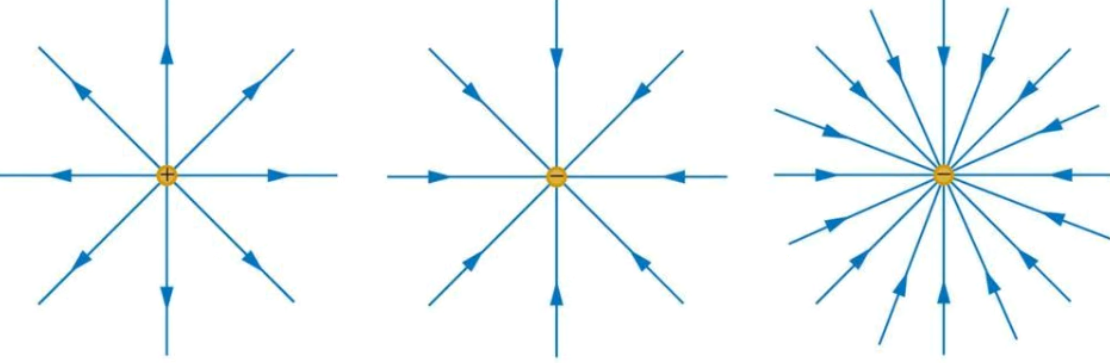
\includegraphics[width=0.75\textwidth]{fieldlines}
\end{figure}
\begin{itemize}
    \item{Like charges repel, opposite charges attract}
    \item{The field is stronger the closer to the source charge it is}
    \item{We \textbf{always} use a \hl{small positive test charge} to map/draw the electric field}
\end{itemize}

\subsection{Rules}
\begin{itemize}
    \item{The lines must originate on a positive charge and end on a negative charge (\hl{positive to negative})}
    \item{The electric field line must be \hl{perpendicular to the surface} of the charge}
    \item{The \hl{number of lines} drawn leaving a positive charge or approaching a negative charge is proportional to the \hl{magnitude of the charge}}
    \item{\hl{No two field lines can cross} each other}
\end{itemize}

\subsection{Electric Field Around A Positive v/s Negative Source Charge}
\begin{figure}[H]
    \centering
    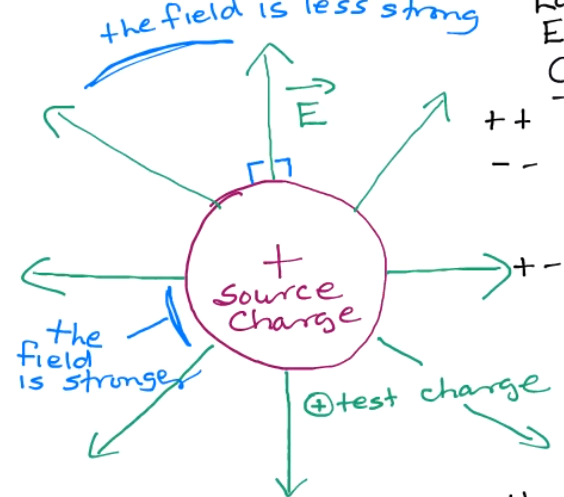
\includegraphics[width=0.4\textwidth]{lines}
    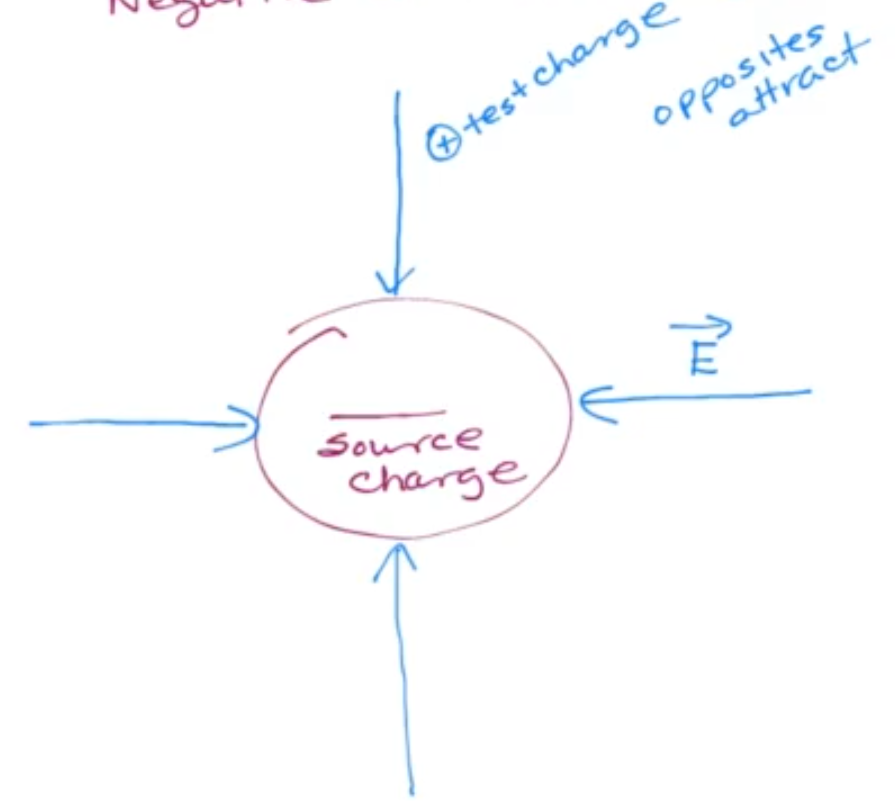
\includegraphics[width=0.4\textwidth]{lines2}
\end{figure}

\subsection{Electric Field Interactions}
\begin{figure}[H]
    \centering
    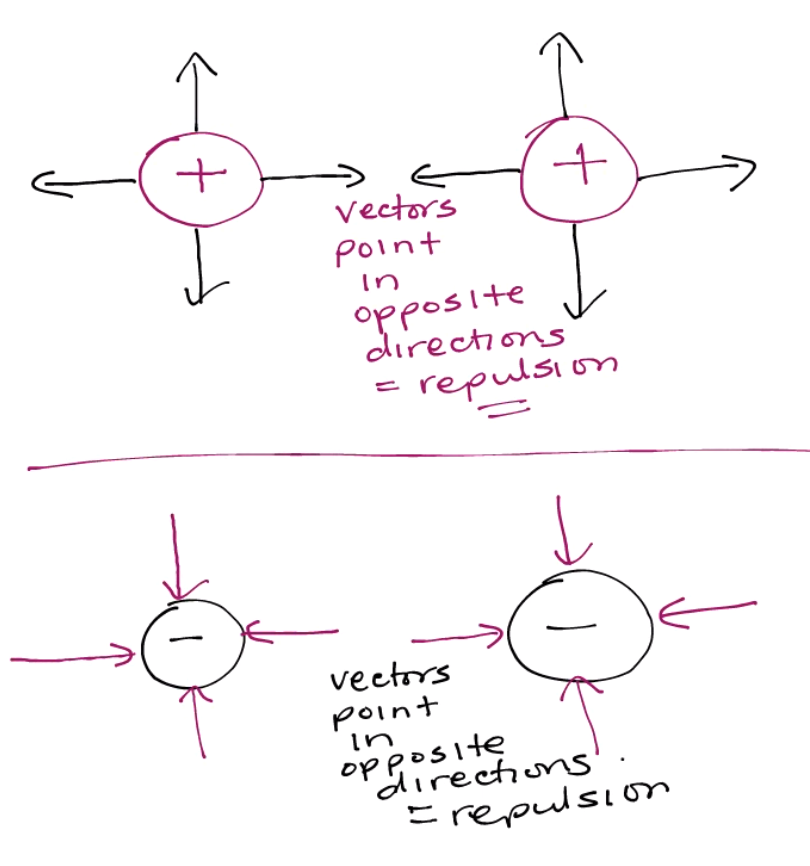
\includegraphics[width=0.4\textwidth]{repel}
    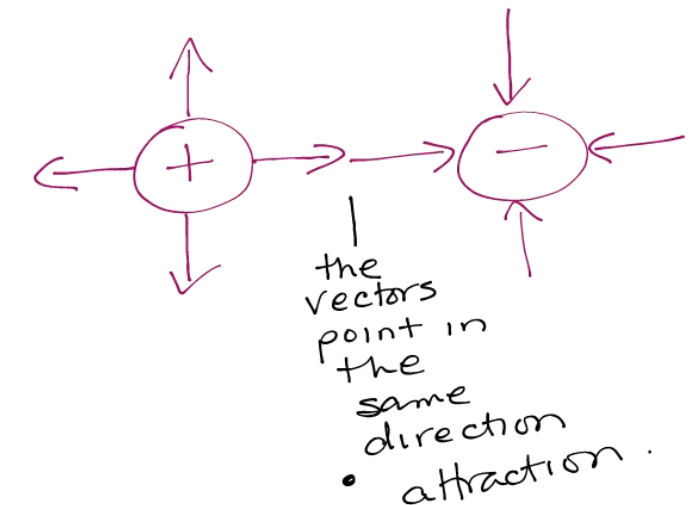
\includegraphics[width=0.4\textwidth]{attract}
\end{figure}

Use this theory with a test particle to determine the direction of an electric field. NOT signs.

For forces, NEVER use negatives for charges ($q$) in formulas. After you calculate a value with no negative charges, look at the signs. If they are same sign, the force is repel. If they are opposite sign, the force is attractive.

\section{Particles}
\begin{figure}[H]
    \centering
    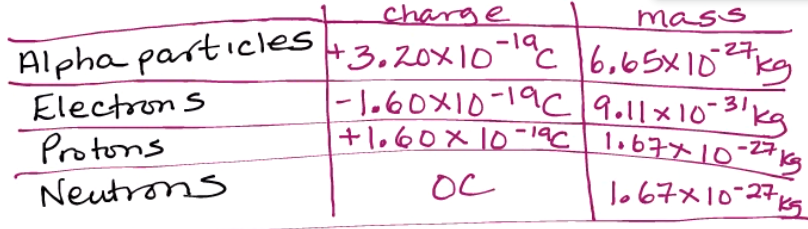
\includegraphics[width=\textwidth]{particles}
\end{figure}

\section{Electric Field Strength}
\subsection{Electric Field Around A Producer (Source Charge)}
\Large $$|\vec{E}| = \frac{kq}{r^2}$$ \normalsize
$$\textrm{Units: } \si{\newton\per\coulomb} \textrm{ or } \si{\V\per\m}$$
\begin{itemize}
    \item{$k$ = Coulomb's Constant (\SI{8.99e9}{\newton\cdot\m\squared\per\coulomb\squared})}
    \item{$q$ = Value of the source charge (\si{\coulomb})}
    \item{$r$ = Distance from the source charge (\si{\m})}
\end{itemize}

\subsection{Electric Field Experienced By A Charge}
\Large $$\vec{E} = \frac{\vec{F}_e}{q}$$ \normalsize
\begin{itemize}
    \item{$\vec{E}$ = Electric Field (\si{\newton\per\coulomb})}
    \item{$\vec{F}_e$ = Electrostatic Force (\si{\newton})}
    \item{$q$ = Test Charge (in a field question, its not source charge) (\si{\coulomb})}
\end{itemize}

\subsection{Example}
Calculate the electric field \SI{2.00}{\cm} from an alpha particle.
$$|\vec{E}| = \frac{(\SI{8.99e9}{\newton\cdot\m\squared\per\coulomb\squared})(\SI{3.20e-19}{\coulomb})}{(\SI{2.00e-2}{\m})^2}$$
$$|\vec{E}| = \SI{7.19e-6}{\newton\per\coulomb} \textrm{ radially outward}$$
\begin{figure}[H]
    \centering
    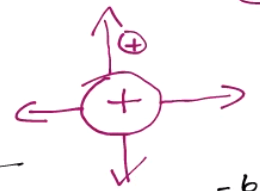
\includegraphics[width=0.3\textwidth]{fieldquestion}
\end{figure}

\subsection{Example II}
Calculate the electric field strength at a point in space where a \SI{3.24e-6}{\coulomb} charge experiences an electrostatic force of \SI{5.29e-3}{\newton}.
$$\vec{E} = \frac{\vec{F}_e}{q}$$
$$\vec{E} = \frac{\SI{5.29e-3}{\newton}}{\SI{3.24e-6}{\coulomb}}$$
$$\vec{E} = \SI{1.63e3}{\newton\per\coulomb}$$

\pagebreak
\subsection{Example III}
Calculate the electric field midway between the two charges below if they are \SI{5.00}{\cm} apart.
\begin{figure}[H]
    \centering
    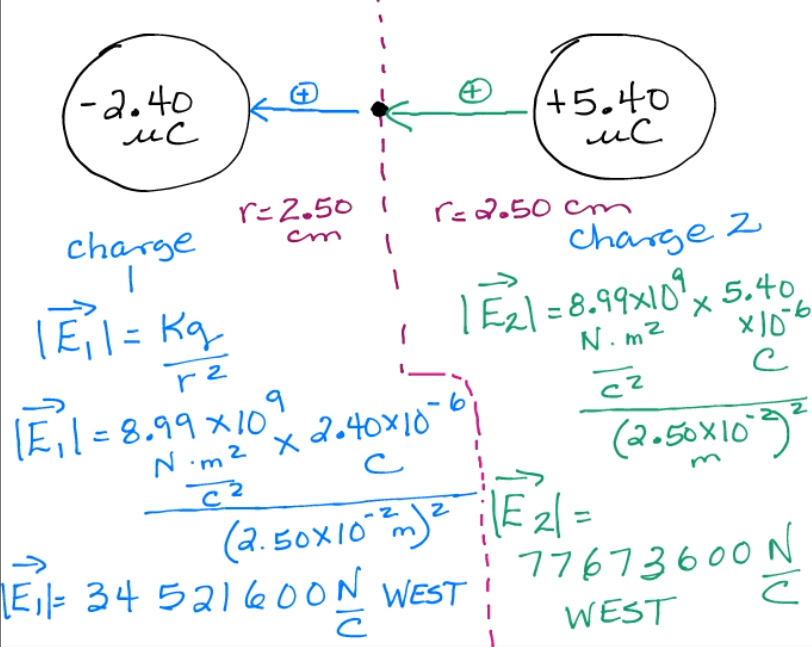
\includegraphics[width=\textwidth]{fieldquestion3}
\end{figure}

$$|\vec{E}_{net}| = |\vec{E}_1| + |\vec{E}_2|$$
$$|\vec{E}_{net}| = \SI{34521600}{\newton\per\coulomb}\textrm{, west} + \SI{77673600}{\newton\per\coulomb}\textrm{, west}$$
$$|\vec{E}_{net}| = \SI{1.12e8}{\newton\per\coulomb}\textrm{, west}$$

\pagebreak
\subsection{Electric Field Around A Producer in Two Dimensions}
\begin{itemize}
    \item{Calculate $\vec{E}$ of the hypotenuse}
    \item{Use trig to get the components of the electric field vector on each side}
\item{
    Direction of the vector is determined by the source charge like before
        \begin{itemize}
            \item{if positive, towards test charge/point (repel)}
            \item{if negative, from test charge/point to source charge (attract)}
        \end{itemize}
    }
    \item{Add the $x$ and $y$ components, positive or negative depending on direction}
    \item{You are left with the components of the net electric field vector}
\end{itemize}

\subsubsection{Example I}
\begin{figure}[H]
    \centering
    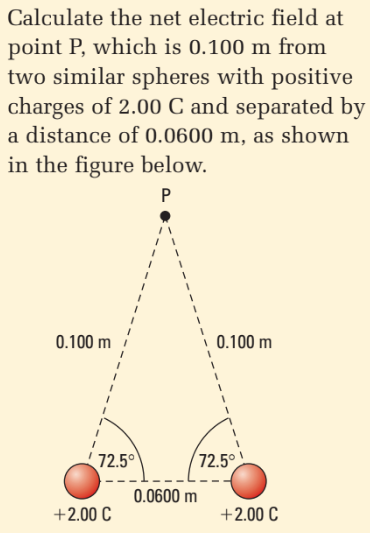
\includegraphics[width=0.3\textwidth]{fieldtriangle}
\end{figure}
$$= \SI{3.43e12}{\newton\per\coulomb}$$

\pagebreak
\section{Electric Field Between Plates}
\Large $$\vec{E} = \frac{V}{d}$$ \normalsize
\begin{itemize}
    \item{$V$ = total voltage across the plate (\si{\volt})}
    \item{$d$ = total distance between the plates (\si{\meter})}
\end{itemize}

\begin{figure}[H]
    \centering
    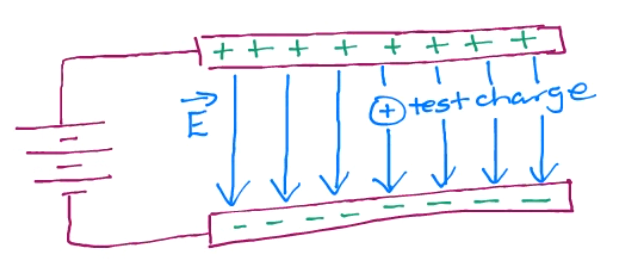
\includegraphics[width=0.50\textwidth]{plate}
\end{figure}

\begin{itemize}
    \item{The electric field between \hl{charged parallel plates} is \hl{uniform} --- identical at any point}
    \item{To determine the \hl{direction} of the electrical field between charged parallel plates, use a \hl{small positive test charge}}
    \item{
        Don't forget that \hl{work is equal to $\SI{0}{\joule}$} if the $F_e$ and $d$ are \hl{not along the same line}
        \begin{itemize}
            \item{$\theta$ (in $W = Fd\cos{\theta}$) must be either\\\ang{0} (force and distance same direction) or \\\ang{180} (force and distance opposite directions)}
        \end{itemize}
    }
\end{itemize}

\subsection{Example}
Two parallel plates are connected to a \SI{12.0}{\volt} battery. If the plates are \SI{6.00e-2}{\m} apart, calculate the electric field strength between them.
$$\vec{E} = \frac{\SI{12.0}{\volt}}{\SI{6.00e-2}{\m}} = \SI{200}{\volt\per\m}$$

\subsection{Example II}
\begin{figure}[H]
    \centering
    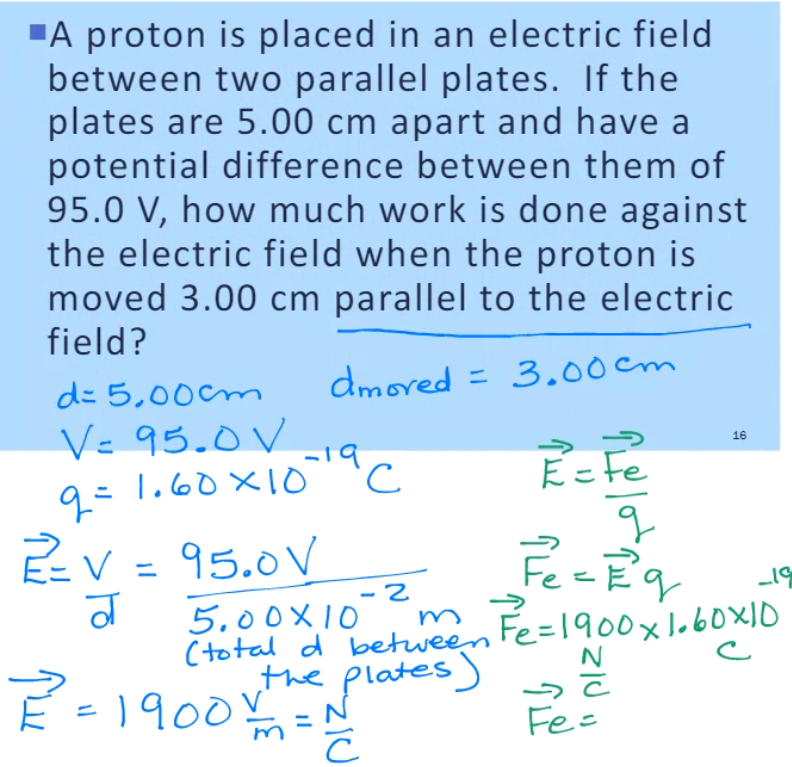
\includegraphics[width=0.39\textwidth]{workplate1}
    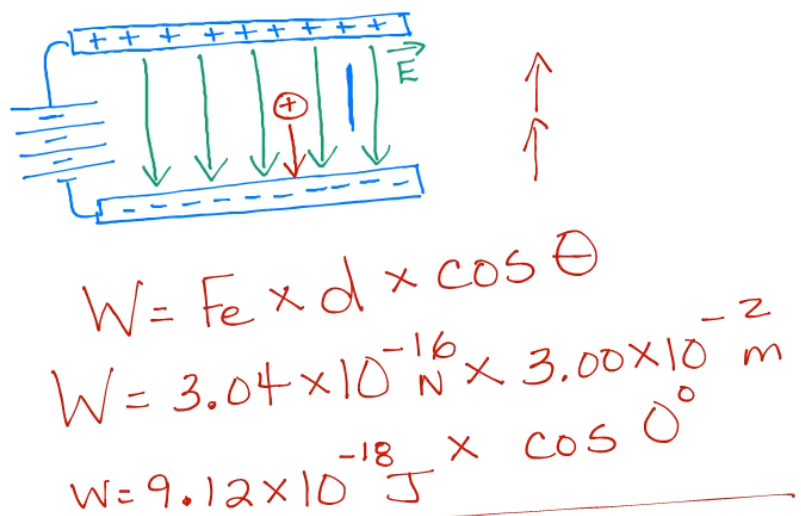
\includegraphics[width=0.5\textwidth]{workplate2}
\end{figure}

\subsection{Example III (Projectile Motion Style)}
An electron beam enters the region between two oppositely charged parallel plates near the negatively charged plate, as shown below. The plates are \SI{0.250}{\m} long and are \SI{0.0500}{\m} apart. There is an electrical potential difference of \SI{120}{\volt} across the two plates as the beam exits the region between the parallel plates. The path of the electrons just touches the edge of one of the plates as the beam exits the region between the parallel plates. \\Determine the minimum initial speed of an electron in the beam. \\Show the direction of the electric field and explain why.
\begin{figure}[H]
    \centering
    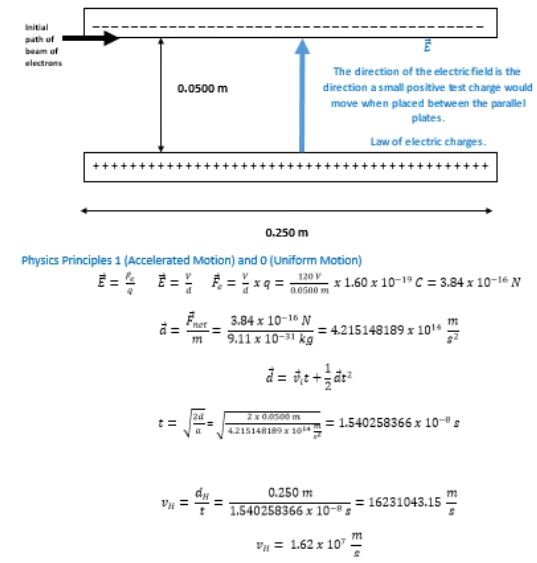
\includegraphics[width=\textwidth]{particleplates}
\end{figure}

\section{Electric Field as a Function of r Graph}
\begin{itemize}
    \item{Make sure all values are times ten to the power of the same exponent before you plot}
\end{itemize}

\begin{figure}[H]
    \centering
    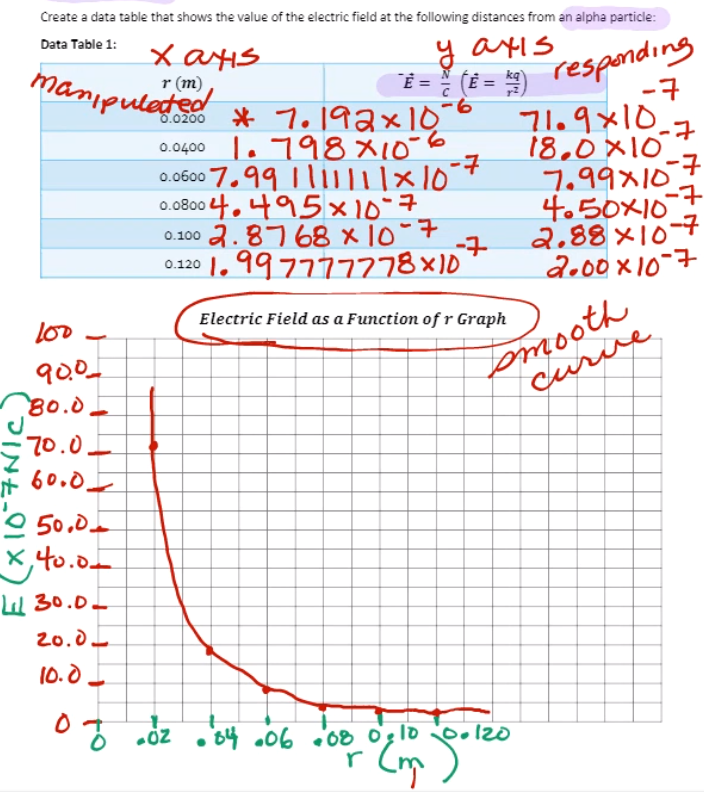
\includegraphics[width=0.75\textwidth]{graph1}
\end{figure}

In order to get a graph that is a straight line, set the $x$ to whatever is proportional to $y$. In this case, $E \propto \frac{1}{r^2}$

\begin{figure}[H]
    \centering
    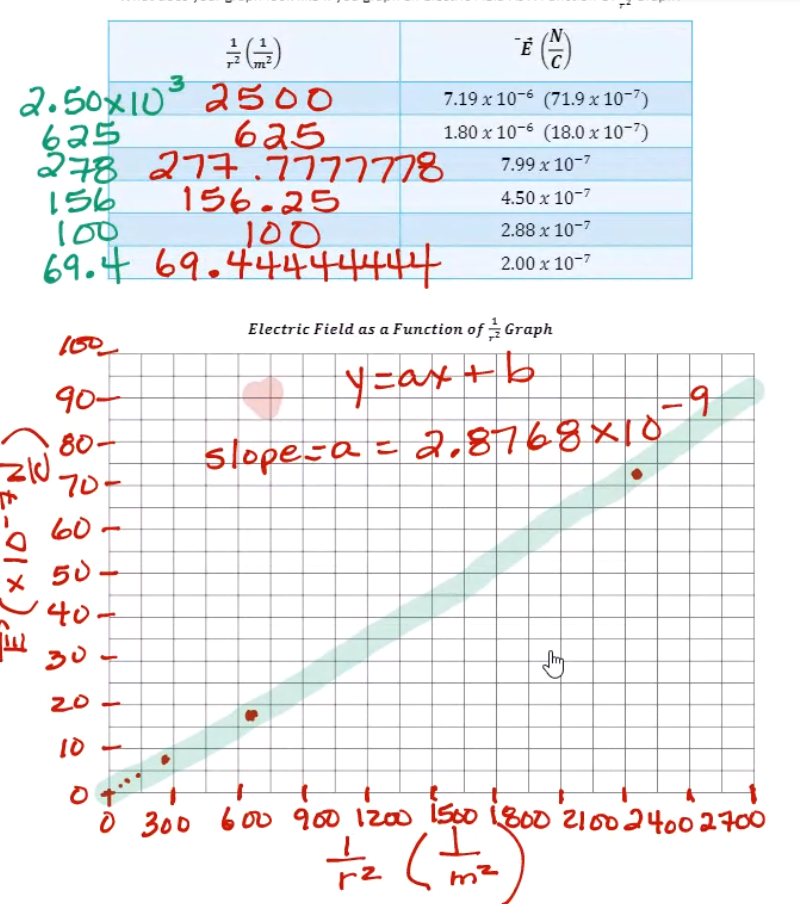
\includegraphics[width=0.75\textwidth]{graph2}
\end{figure}

Use the slope of this graph in further calculations.

slope = $\frac{E}{\frac{1}{r^2}} = Er^2$

You can substitute the slope into anywhere with $Er^2$.

These exact things also work for force as a function of separation distance graphs.\\$m = \frac{F}{\frac{1}{r^2}} = Fr^2$

\subsection{Slope}
Use your graphing calculator functions to calculate slope. (lists)

$$m = \frac{\Delta{y}}{\Delta{x}} = \frac{y_f - y_i}{x_f - x_i}$$

If you don't have a graphing calculator, manually calculate slope. Make sure to select points off the graph line that are \hl{not plotted points}.

\pagebreak
\section{Coulomb's Law}
\Large $$|\vec{F}_e| = \frac{kq_1q_2}{r^2}$$ \normalsize
$$F_e \propto q_1q_2 \qquad F_e \propto \frac{1}{r^2}$$

The magnitude of the electrostatic force of interaction between two point charges is directly proportional to the \textbf{scalar multiplication} of the magnitudes of charges and inversely proportional to the square of the distance between them.

Most questions are simply just plugging in the data you're given and solving for a variable.

\subsection{Data Miner Question}
\begin{itemize}
    \item{If two charges have \hl{brief contact}, the charges will evenly distribute}
    \item{Add the charges together and divide by two}
    \item{Both will share this new charge if the objects are same size and material, which it always will be at the Physics 30 level}
    \item{Some questions ask for the speed/acceleration of charged objects. For these questions, remember that $F_e = F_c$, and $F_c = ma_c$ (which is on your formula sheet) (this doesn't apply to parallel plates questions)}
\end{itemize}

\subsubsection{Example}
A \SI{7.50}{\micro\coulomb} charge and a \SI{-9.24}{\micro\coulomb} charge are brought into \textbf{brief contact}, then moved \SI{1.75}{\cm} away from each other. Calculate the electrostatic force between the two charges.
$$\SI{7.50e-6}{\coulomb} + \SI{-9.24e-6}{\coulomb} = \SI{-1.74e-6}{\coulomb}$$
$$\SI{-1.74e-6}{\coulomb} \div 2 = \SI{-8.70e-7}{\coulomb}$$

$$|\vec{F}_e| = \frac{(\SI{8.99e9}{\newton\cdot\m\squared\per\coulomb\squared})(\SI{8.70e-7}{\coulomb})(\SI{8.70e-7}{\coulomb})}{(\SI{1.75e-2}{\m})^2}$$
$|\vec{F}_e| = \SI{22.2}{\newton} \textrm{ repulsive}$ (like charges repel)

\subsection{Long Answer Example}
An electron and a proton in the hydrogen atom are separated by \SI{5.29e-11}{\m} when the electrion is in the first Bohr orbit.
\\a) Calculate $\vec{F}_g$ between the electron and proton.
\\b) Calculate $\vec{F}_e$ between the electron and proton.
\\c) Which force, $\vec{F}_g$ or $\vec{F}_e$, is responsible for the electron orbiting the nucleus? Why?
\\d) Calculate the speed of the electron as it orbits the nucleus.
\\e) Calculate the period of the electron.

\begin{figure}[H]
    \centering
    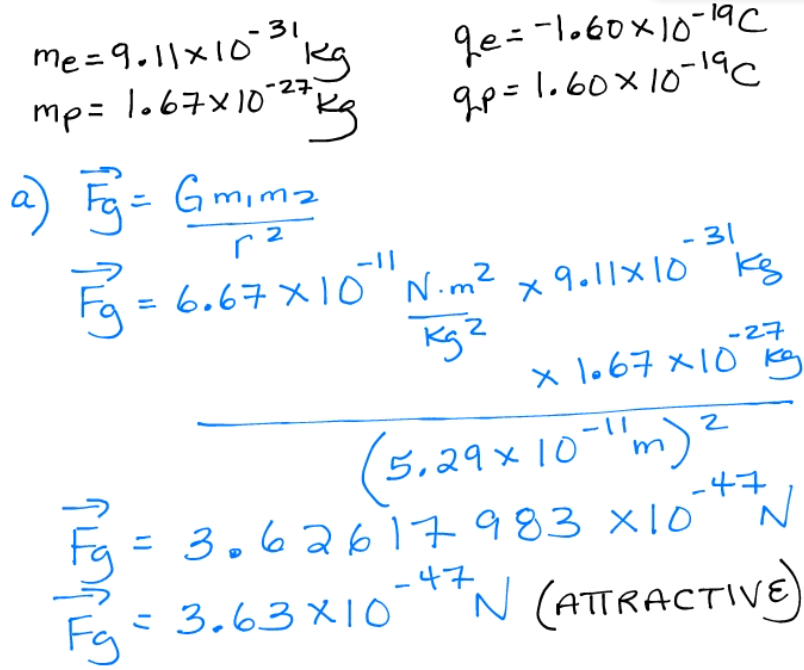
\includegraphics[width=0.45\textwidth]{longa}
    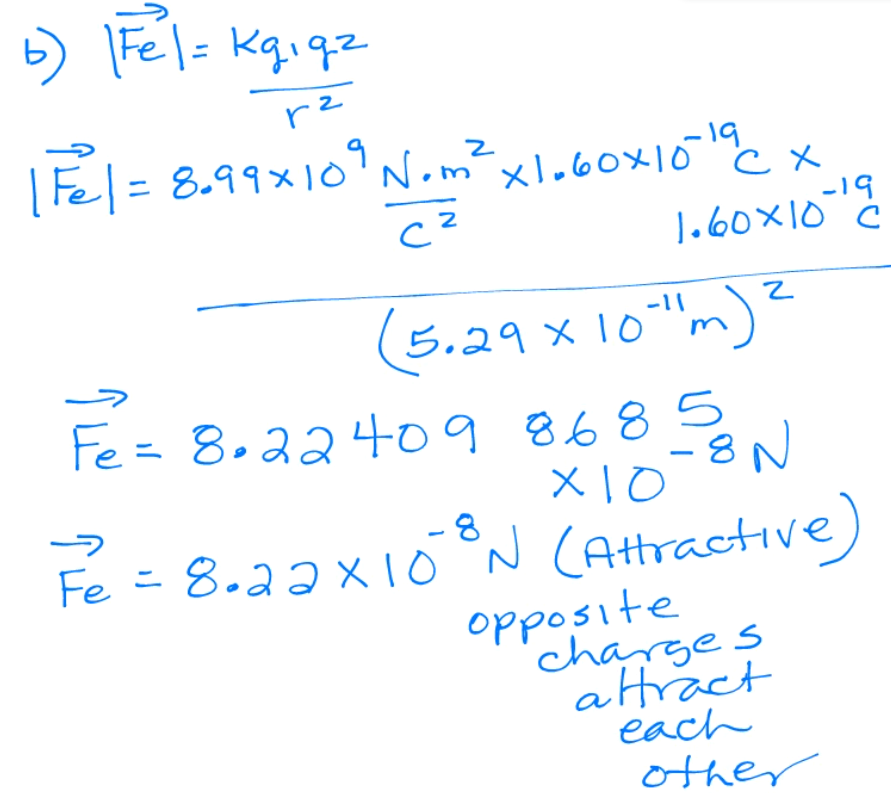
\includegraphics[width=0.45\textwidth]{longb}
\end{figure}
c) $\vec{F}_e$ is responsible for the electron's orbit as it is significantly larger than $\vec{F}_g$.
\begin{figure}[H]
    \centering
    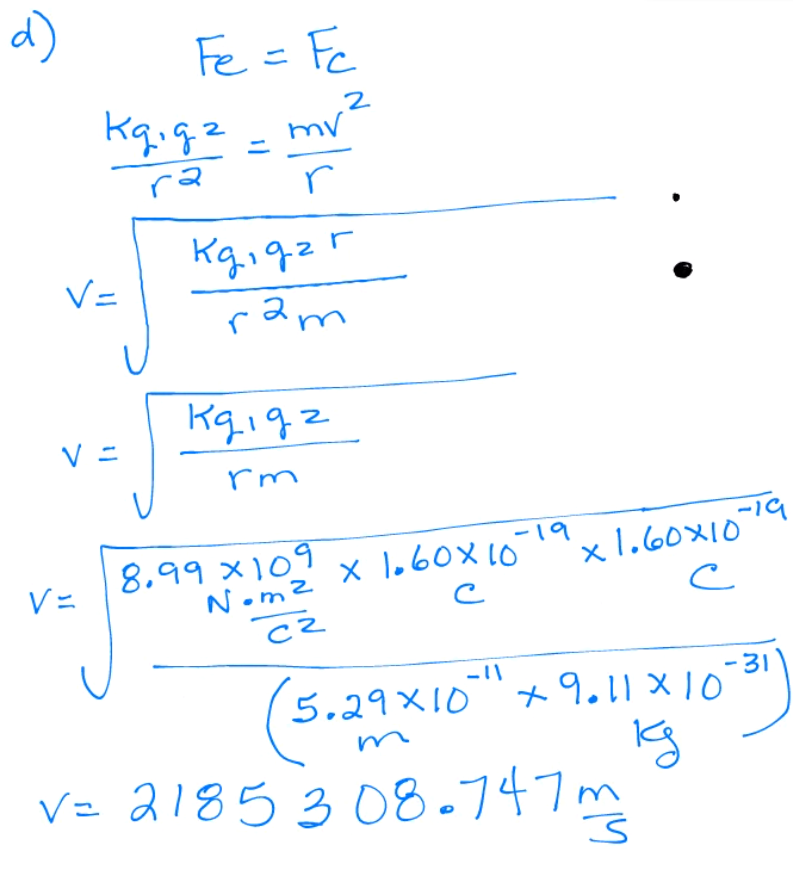
\includegraphics[width=0.45\textwidth]{longd}
    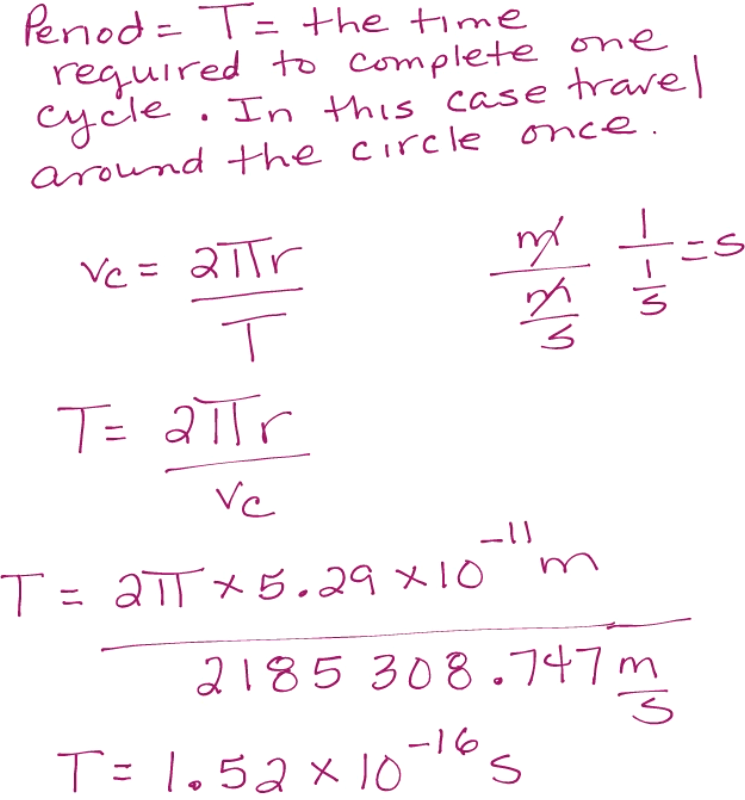
\includegraphics[width=0.45\textwidth]{longe}
\end{figure}

\pagebreak
\subsection{Multiple Charges Example}
Calculate the $F_e$ exerted on charge B due to charges A and C.
\begin{figure}[H]
    \centering
    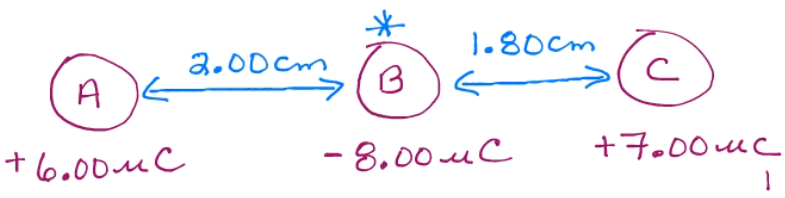
\includegraphics[width=0.50\textwidth]{Fequestion}
\end{figure}
\begin{figure}[H]
    \centering
    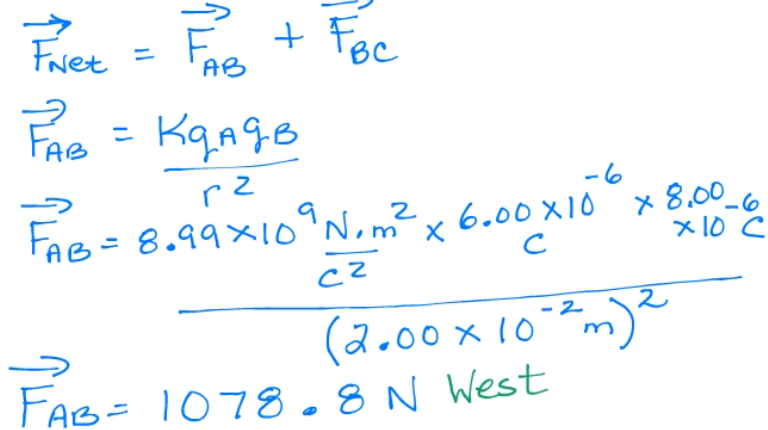
\includegraphics[width=0.45\textwidth]{Fequestion2}
    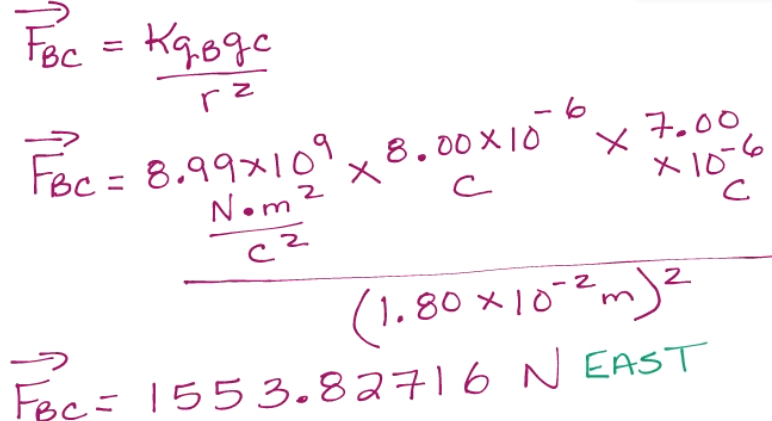
\includegraphics[width=0.45\textwidth]{Fequestion3}
    \caption{The direction of each force is where the reference charge (charge B) is going to move. \\For instance, A and B are opposite charges, they'll attract. A is on the west of B, so the force is west.}
    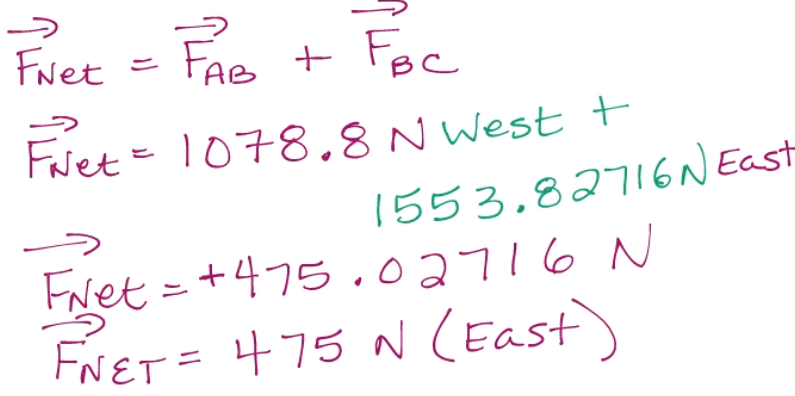
\includegraphics[width=0.75\textwidth]{Fequestion4}
\end{figure}

\subsection{Multiple Charges Example I}
\begin{figure}[H]
    \centering
    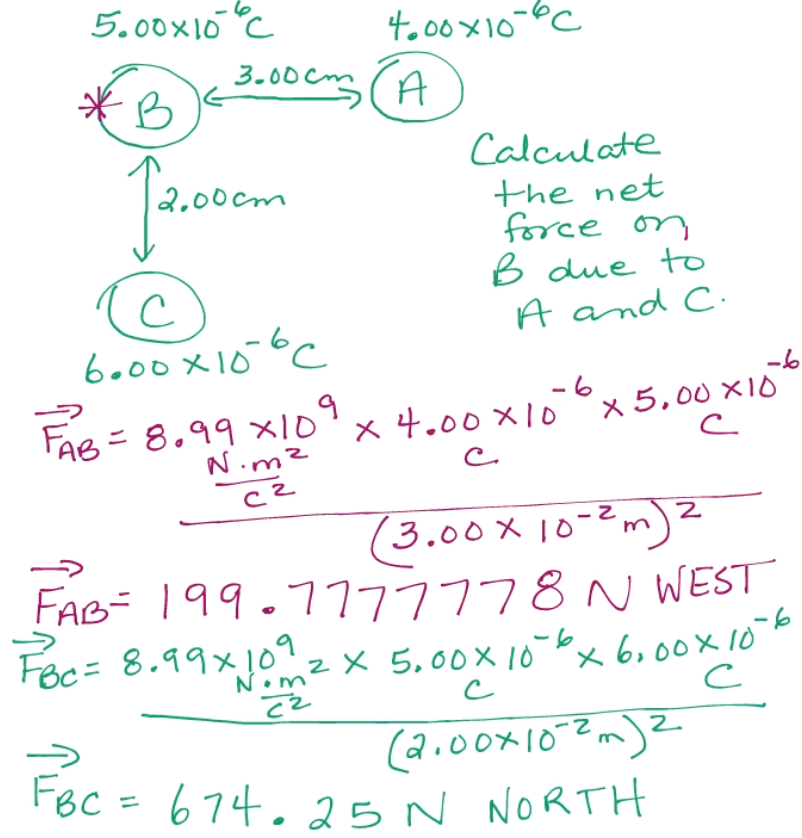
\includegraphics[width=0.7\textwidth]{multiple}
    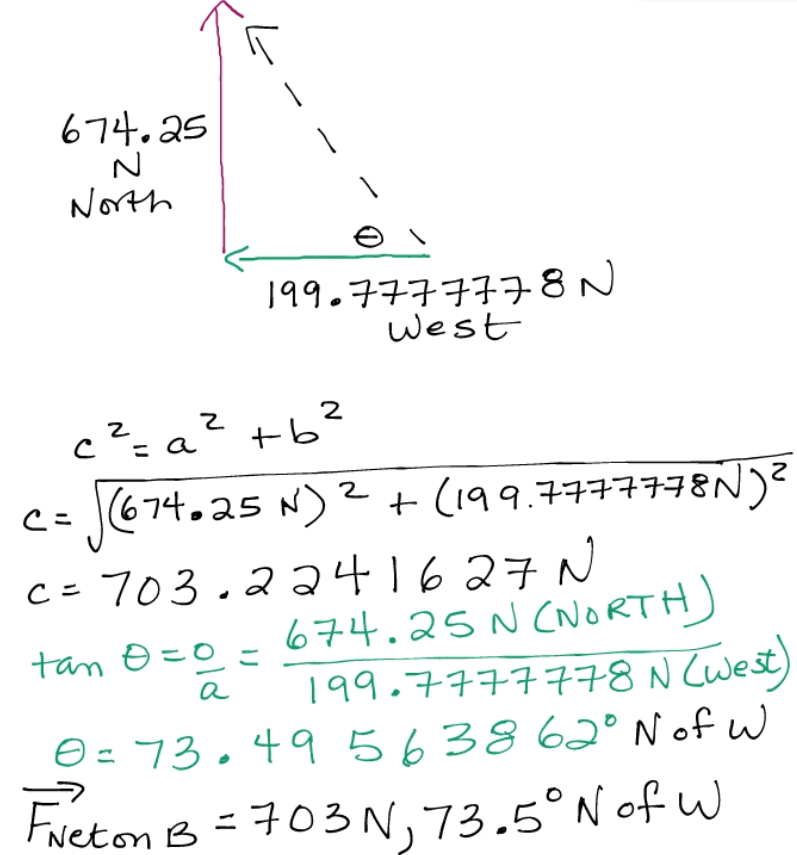
\includegraphics[width=0.7\textwidth]{multiple2}
\end{figure}

\end{document}
